\documentclass{beamer}

\usetheme{Madrid}

\usepackage[utf8]{inputenc}
\usepackage[T1]{fontenc}
\usepackage{amsmath}
\usepackage{amsfonts}
\usepackage{amssymb}
\usepackage{tikz}
\usetikzlibrary{quantikz}
\usepackage{lineno}
\usepackage{multirow}

\title{Quantum Computing and Cryptography}
\author{Damien, Théo, Matthieu}
\institute{University}
\date{February 12, 2025}

\begin{document}

\begin{frame}
\maketitle
\end{frame}

\begin{frame}{Outline}
\tableofcontents
\end{frame}

\section{Intro}
\begin{frame}{Introduction}
\begin{linenumbers}
	\begin{itemize}
		\item Cryptography=TODO
		\item TODO: secret
		\item<2->[$\rightarrow$] Science of secret
	\end{itemize}
\end{linenumbers}
\end{frame}

\section{RSA}
\begin{frame}{RSA}
\begin{linenumbers}

\end{linenumbers}
\end{frame}

\section{Quantum computing}

\subsection{Introduction to the quantum world}
\subsubsection*{Qubits}
\begin{frame}{Qubits}
\begin{linenumbers}
	\begin{block}<+->{Classical bit}
		$b \in \{0, 1\}$
		\begin{itemize}[<+->]
			\item $0$
			\item $1$
		\end{itemize}
	\end{block}

	\begin{block}<+->{Quantum bit}
		$\ket{\psi} \in \mathbb{C}^2$
		\begin{columns}[T,onlytextwidth]
			\column{0.5\textwidth}
				\begin{itemize}[<+->]
					\item $\ket{0} = \begin{bmatrix} 1 \\ 0 \end{bmatrix}$
					\item $\ket{1} = \begin{bmatrix} 0 \\ 1 \end{bmatrix}$
				\end{itemize}
			\column{0.5\textwidth}
				\begin{itemize}[<+->]
					\item $\ket{+} = \frac{1}{\sqrt{2}}\begin{bmatrix} 1 \\ 1 \end{bmatrix}$
					\item $\ket{-} = \frac{1}{\sqrt{2}}\begin{bmatrix} 1 \\ -1 \end{bmatrix}$
				\end{itemize}
		\end{columns}
	\end{block}
\end{linenumbers}
\end{frame}


\subsubsection*{Mesures}
\begin{frame}{Mesures}
\begin{linenumbers}
  \begin{itemize}[<+->]
    \item $\bra0$ => 0 (100\%)
    \item $\bra1$ => 1 (100\%)
    \item $\bra+$ => 0 (50\%), 1 (50\%)
    \item $\bra-$ => 0 (50\%), 1 (50\%)
  \end{itemize}
\end{linenumbers}
\end{frame}

\subsubsection*{Gates}
\begin{frame}{Gates - Slide 1}
\begin{linenumbers}
    \begin{itemize}[<+->]
        \item Gate $X$
        \begin{itemize}
            \item $X\ket{0} \rightarrow \ket{1}$
            \item $X\ket{1} \rightarrow \ket{0}$
        \end{itemize}
        \item Circuit
        \begin{quantikz}
            \lstick{$\ket{0}$} & \gate{X} & \meter{}
        \end{quantikz}
    \end{itemize}
\end{linenumbers}
\end{frame}

\begin{frame}{Gates - Slide 2}
\begin{linenumbers}
    \begin{itemize}[<+->]
        \item Gate $H$
        \begin{itemize}
            \item $H\ket{0} \rightarrow \ket{+}$
            \item $H\ket{1} \rightarrow \ket{-}$
        \end{itemize}
        \item Circuit
        \begin{quantikz}
            \lstick{$\ket{0}$} & \gate{H} & \meter{}
        \end{quantikz}
    \end{itemize}
\end{linenumbers}
\end{frame}

\subsection{Quantum algorithms}
\subsubsection*{Problème B.V}
\begin{frame}{Problème B.V}
\begin{linenumbers}
Given the oracle of a function $f$ :

$f : \{0, 1\}^n \rightarrow \{0, 1\}$
$f(x) = x\cdot s$

Find $s$ in the few request possible.
\end{linenumbers}
\end{frame}

\subsubsection*{Algo classique}
\begin{frame}{Algo classique - Slide 1}
\begin{linenumbers}
with $n=2$
try :
\begin{itemize}[<+->]
    \item $f(10) = s_0$
    \item $f(01) = s_1$
\end{itemize}

2 requests.
\end{linenumbers}
\end{frame}

\begin{frame}{Algo classique - Slide 2}
\begin{linenumbers}
in general :
$\mathcal{O}(n)$ $\rightarrow$ Try every $x$ that contains one bit to 1. At each query, we get the value of that bit in s
\end{linenumbers}
\end{frame}

\subsubsection*{Algo Quantique}
\begin{frame}{Algo Quantique - Slide 1}
\begin{linenumbers}
$\mathcal{O}(1)$ $\rightarrow$ Just try every $x$ at the same time.

Not only the $x$ with only one bit at one but every possible $x$.
\end{linenumbers}
\end{frame}

\begin{frame}{Algo Quantique - Slide 2}
\begin{linenumbers}
\begin{quantikz}
    \lstick{$\ket{0}$} & \gate{H} & \qw & \qw & \gate{H} & \meter{} \\
    \lstick{$\ket{0}$} & \gate{H} & \ctrl{-1} & \gate{H} & \qw & \meter{}
\end{quantikz}
\end{linenumbers}
\end{frame}

\subsubsection*{Shor}
\begin{frame}{Shor}
\begin{linenumbers}
    \begin{itemize}[<+->]
        \item Gain de complexité :
        $\mathcal O(e^b)$ $\rightarrow$ $\mathcal O(b³)$
        \item combien de qubit il faut
        \item combien de cubit on as
    \end{itemize}
\end{linenumbers}
\end{frame}

\section{Post-Quantum cryptography}
\subsection{Intro to PQ cryptography}
\begin{frame}{What is PQ cryptography}
\begin{linenumbers}
	\begin{itemize}
		\item Based on (other) mathematical problems
		\item Considered unsolvable by a quantum computer
	\end{itemize}

	What it is not :
	\begin{itemize}
		\item Cryptography \textbf{using} quantum technologies
	\end{itemize}
\end{linenumbers}
\end{frame}

\begin{frame}{The problems}
	\begin{itemize}
		\item Codes
		\item Hash functions
		\item Multivariates polynomials systems
		\item Isogenies
		\item {\color<2>{red} Lattices}
	\end{itemize}
\end{frame}

\begin{frame}{Why lattices ?}
	\begin{itemize}
		\item Well spread
		\item Good results
			\begin{table}[h!]
			\begin{tabular}{|c|c|}
				\hline
				\multicolumn{2}{|c|}{Encryption/Key encapsulation} \\
				\hline
				Crystals-Kyber & Lattices \\
				\hline
				\multicolumn{2}{|c|}{Signatures} \\
				\hline
				Crystals-Dilithium & Lattices \\
				Falcon & Lattices \\
				Sphincs+ & Hash \\
				\hline
			\end{tabular}
			\end{table}
	\end{itemize}
\end{frame}

\subsection{Lattice cryptography}
\begin{frame}{What is a lattice ?}
	\begin{linenumbers}
		\begin{itemize}
			\item A discret subgroup of $RR^n$
		\end{itemize}

		abc akpqzsfkeokf  akozckdp kpzqkfs pkzapqfkpkde pzkpkd czqks qkp kfsdkvoesd, okpze kswkw k
	\end{linenumbers}

	Like vector spaces, we have :
	\begin{itemize}
		\item Vectors and matrices
		\item Linear combination
	\end{itemize}
\end{frame}

\begin{frame}{What is a lattice ? (cont'd)}
	\begin{columns}[t]
	\begin {column}{0.5\textwidth}
		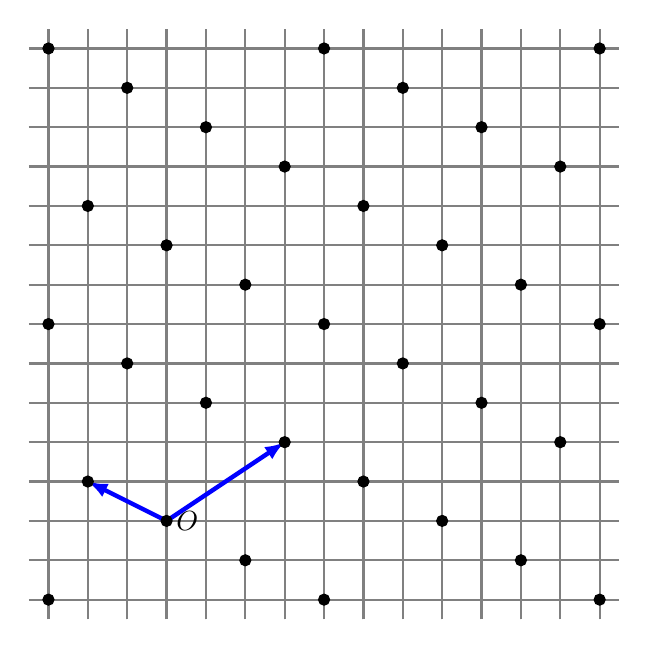
\begin{tikzpicture}
		\foreach \i in {1, ..., 8, 1.5, ..., 7.5} {
			\draw [gray, thick] (\i, 0.75) -- (\i, 8.25);
		}
		\foreach \i in {1, ..., 8, 1.5, ..., 7.5} {
			\draw [gray, thick] (0.75, \i) -- (8.25, \i);
		}

		%%% Basis
		\draw[ultra thick, blue, arrows={-{Latex[length=2.5mm]}}] (2.5, 2) -- (4, 3);
		\draw[ultra thick, blue, arrows={-{Latex[length=2.5mm]}}] (2.5, 2) -- (1.5, 2.5);

		%%% The lattice's points
		\filldraw[black] (8, 1) circle (2pt);

		\filldraw[black] (7, 1.5) circle (2pt);

		\filldraw[black] (4.5, 1) circle (2pt);
		\filldraw[black] (6, 2) circle (2pt); % end
		\filldraw[black] (7.5, 3) circle (2pt);

		\filldraw[black] (3.5, 1.5) circle (2pt);
		\filldraw[black] (5, 2.5) circle (2pt);
		\filldraw[black] (6.5, 3.5) circle (2pt); % end
		\filldraw[black] (8, 4.5) circle (2pt);

		\filldraw[black] (1, 1) circle (2pt); % beg
		\filldraw[black] (2.5, 2) circle (2pt) node[anchor=west]{$O$};
		\filldraw[black] (4, 3) circle (2pt);
		\filldraw[black] (5.5, 4) circle (2pt);
		\filldraw[black] (7, 5) circle (2pt); % end

		\filldraw[black] (1.5, 2.5) circle (2pt); % beg
		\filldraw[black] (3, 3.5) circle (2pt);
		\filldraw[black] (4.5, 4.5) circle (2pt);
		\filldraw[black] (6, 5.5) circle (2pt);
		\filldraw[black] (7.5, 6.5) circle (2pt); % end

		\filldraw[black] (2, 4) circle (2pt); % beg
		\filldraw[black] (3.5, 5) circle (2pt);
		\filldraw[black] (5, 6) circle (2pt);
		\filldraw[black] (6.5, 7) circle (2pt);
		\filldraw[black] (8, 8) circle (2pt); % end

		\filldraw[black] (1, 4.5) circle (2pt);
		\filldraw[black] (2.5, 5.5) circle (2pt); % beg
		\filldraw[black] (4, 6.5) circle (2pt);
		\filldraw[black] (5.5, 7.5) circle (2pt);

		\filldraw[black] (1.5, 6) circle (2pt);
		\filldraw[black] (3, 7) circle (2pt);  % beg
		\filldraw[black] (4.5, 8) circle (2pt);

		\filldraw[black] (2, 7.5) circle (2pt);

		\filldraw[black] (1, 8) circle(2pt);
		\end{tikzpicture}
	\end{column}
	\begin{column}{0.45\textwidth}
		FIXME : Basis:

		\[\left\{\left(\begin{matrix}3\\2\end{matrix}\right), \left(\begin{matrix}-2\\1\end{matrix}\right)\right\}\]
	\end{column}
	\end{columns}
\end{frame}

\begin{frame}{Learning with error problem}
	TODO
\end{frame}

\begin{frame}{(Fully) homomorphic encryption}
	TODO
\end{frame}

\subsection{Limits of PQ cryptography}
\begin{frame}
	Size
	\begin{tabular}{|c|c|}
		\hline
		TODO & \\
		\hline
	\end{tabular}
\end{frame}

\begin{frame}{Not necessarly robust to classical computer}
	\begin{itemize}
		\item Example : Supersingular isogenies Diffie-Hellman key exchange
	\end{itemize}
\end{frame}

\section{Conclusion}
\begin{frame}{Conclusion}
\begin{linenumbers}
    % Content from brouillon.md - To be filled
\end{linenumbers}
\end{frame}

\end{document}
